\chapter{Implementation}
\label{ch:implementation}

\section{Code Structure \& HDL Hierarchy}
Implementation starts from the block diagram described in Chapter \ref{ch:design}, transitioning from the high-level design to laying out the HDL blocks within a skeleton Scala project.

Chisel modules are Scala classes, which allows to use existing standard Scala practices in structuring and developing the code. The code is structured as an sbt project, using a standard Java/Scala package layout \cite{scala_style}. sbt is the industry standard build tool for Scala, providing a DSL for describing the structure and dependencies of the project in the \txt{build.sbt} file, and a command line interface for building, running, and testing the project \cite{sbt}. The sbt template used is one available on GitHub as the standard Chisel sbt template \footnote{\url{https://github.com/freechipsproject/chisel-template}}.

The top-level package is \txt{dev.joeyh.pio} (the author's domain is \txt{joeyh.dev}), containing the following sub-modules and files:

\begin{itemize}
    \item \txt{execution} - The execution unit and sub-components
          \begin{itemize}
              \item \txt{ExecUnit} - The top-level execution unit
              \item \txt{Decode} - Instruction decoder
              \item \txt{ProgramCounter} - PC register
              \item \txt{Branch} - JUMP execution unit
              \item \txt{Move} - MOV/SET execution unit
              \item \txt{Wait} - WAIT execution unit
          \end{itemize}
    \item \txt{fifo} - FIFOs and reusable interface definitions
          \begin{itemize}
              \item \txt{Fifo} - The FIFO module and sub-components, used for both RX and TX FIFOs
              \item \txt{ProducerIO} - Bundle definition for FIFO producer
              \item \txt{ConsumerIO} - Bundle definition for FIFO consumer
          \end{itemize}
    \item \txt{shiftreg} - Shift registers
          \begin{itemize}
              \item \txt{ISR} - Input shift register
              \item \txt{OSR} - Output shift register
              \item \txt{ShiftRegIO} - Common shift register interface definitions
          \end{itemize}
    \item \txt{memory} - Shift registers
          \begin{itemize}
              \item \txt{CSR} - Control and status register file
              \item \txt{InstructionMem} - 32x16bit Instruction memory
              \item \txt{ScratchReg} - 32-bit scratch register
              \item \txt{Pins} - Pin register and I/O mapping
          \end{itemize}
    \item \txt{util} - Miscellaneous reusable components and utilities
          \begin{itemize}
              \item \txt{Random} - functions for generating random Chisel \txt{UInt}s, used for testing
              \item \txt{ReadWrite} - reusable read and write port interface definitions
              \item \txt{ClockDivider} - clock divider module
          \end{itemize}
\end{itemize}

Some files contain one (or more) Chisel modules, while others contain bundle definitions that are designed to be reused accross multiple modules, and others just contain miscellaneous utility or helper objects. The HDL module hierarchy of the overall design from this is fairly flat, shown in Figure \ref {fig:hdl_hierarchy}.

\begin{figure}[H]
    \centering
    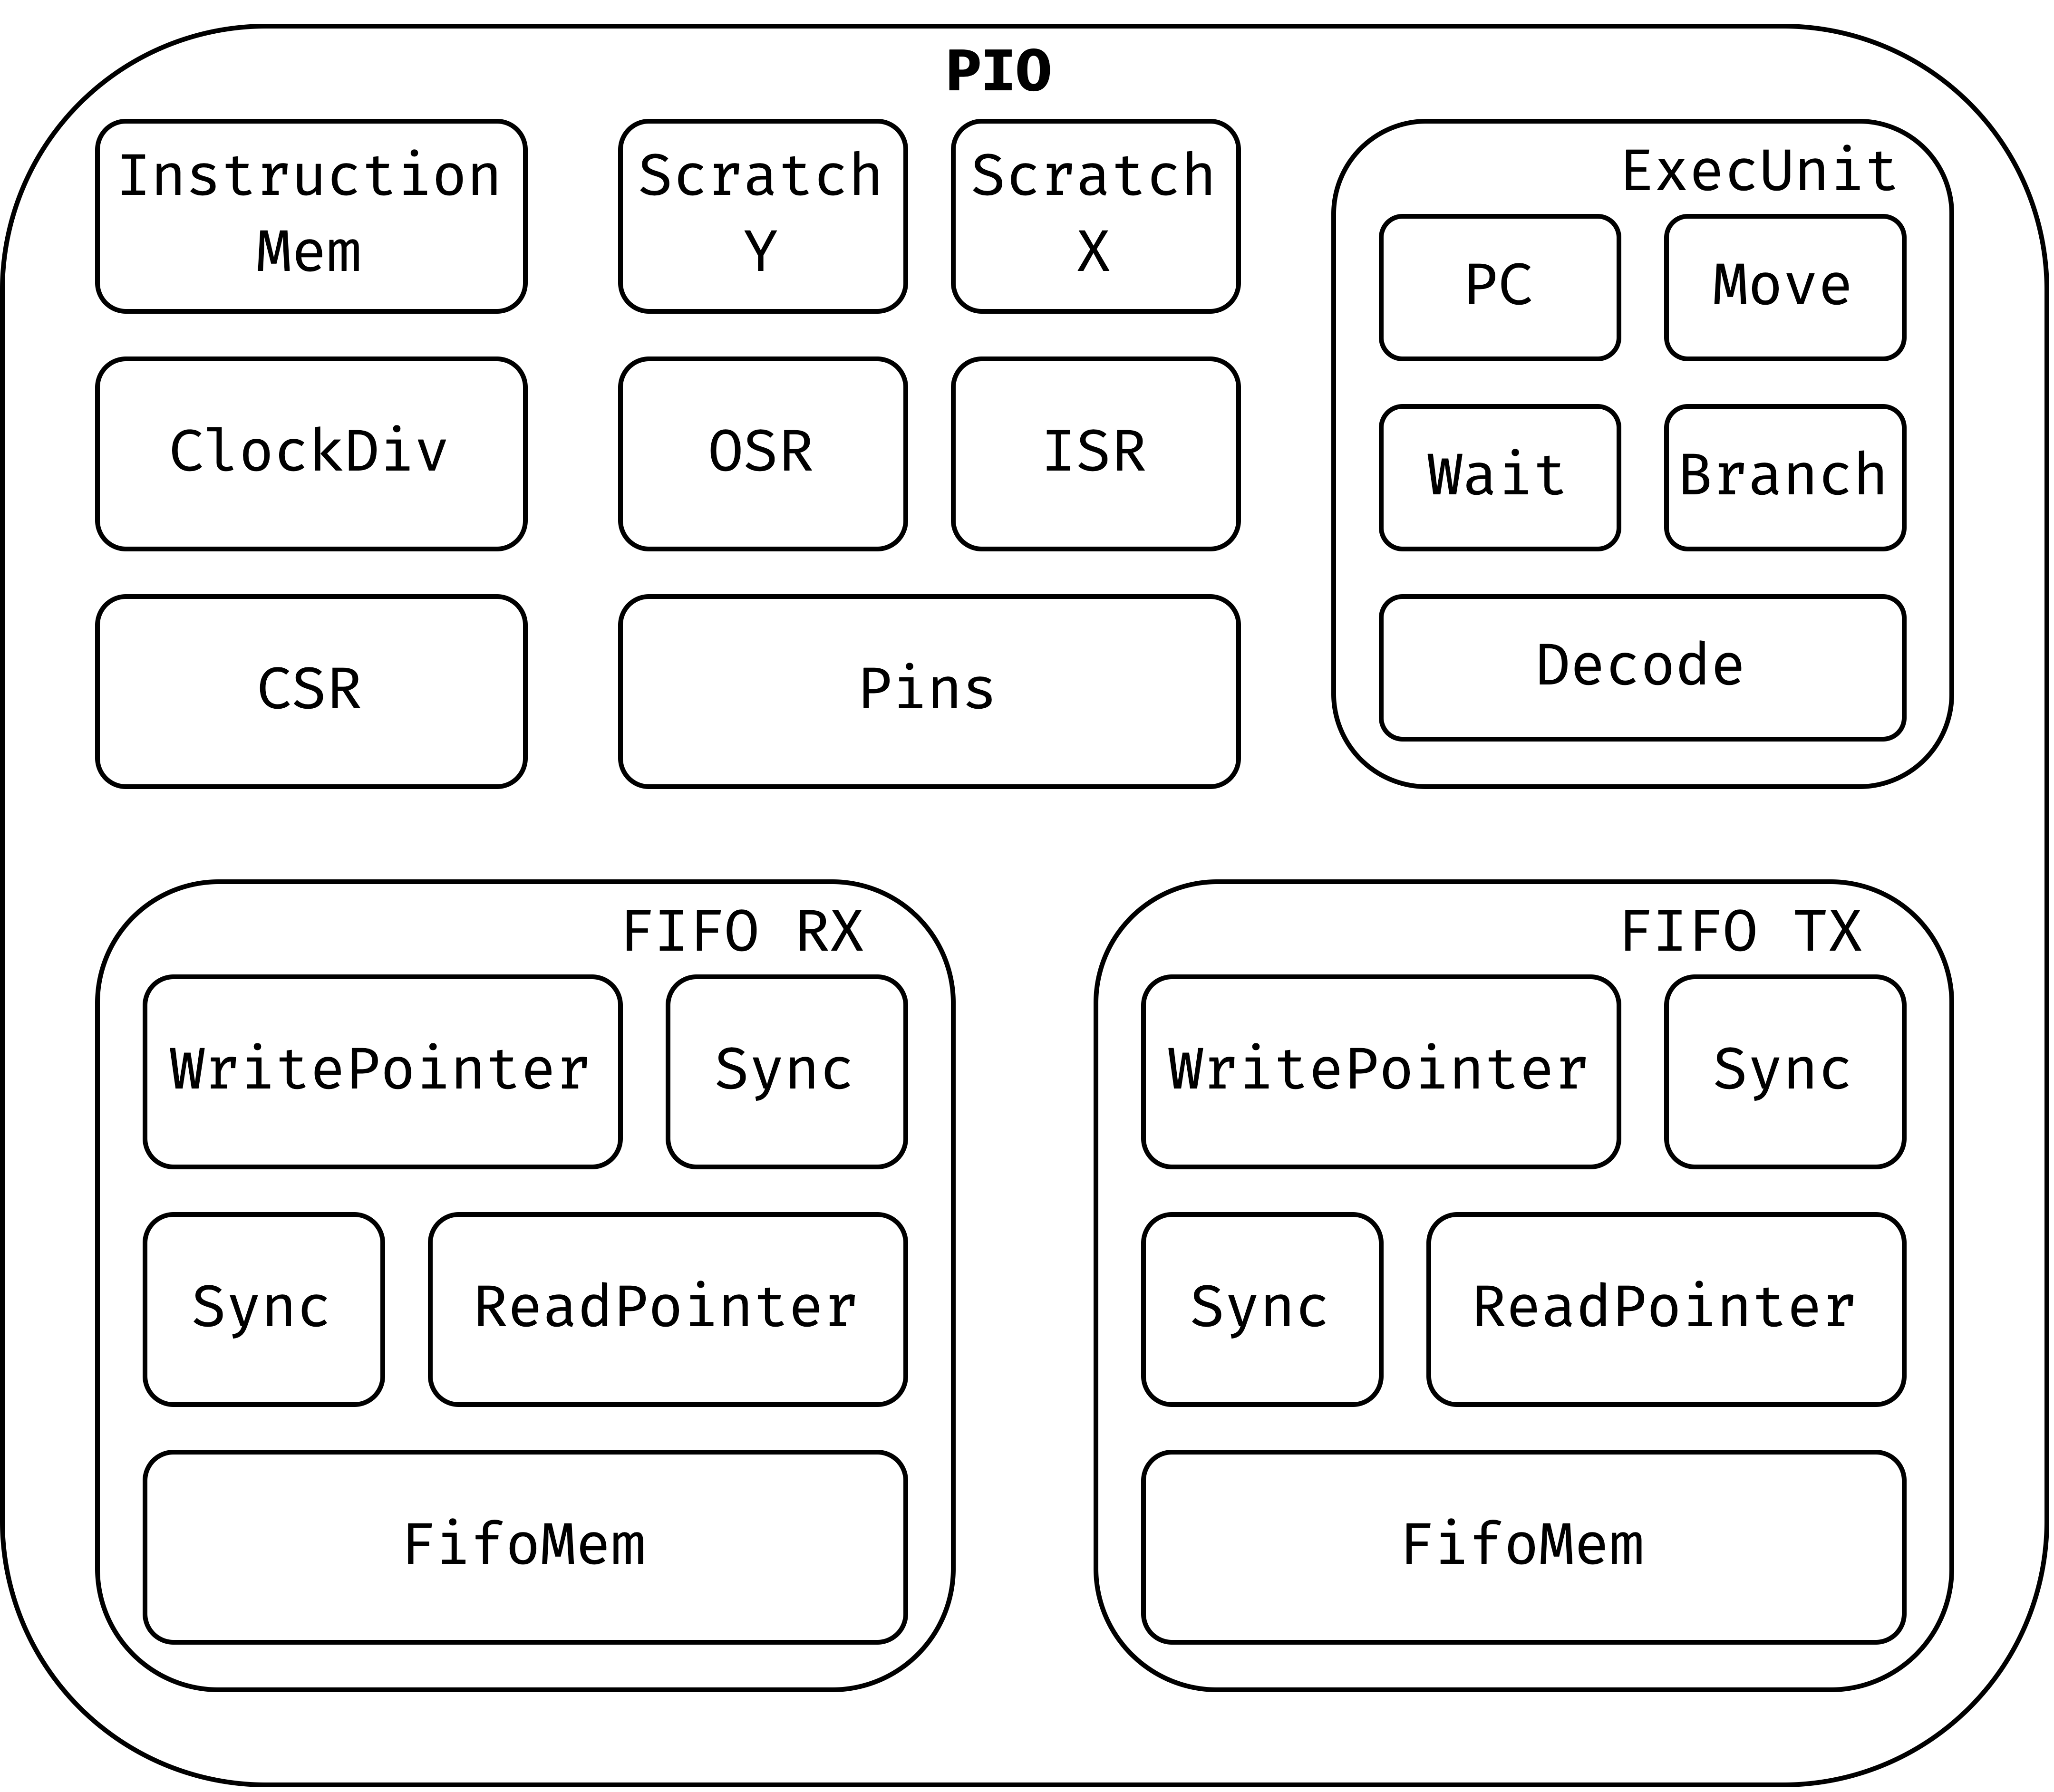
\includegraphics[width=0.7\textwidth]{../img/pio-top.png}
    \caption{The modular, hierarchical design of the PIO.}
    \label{fig:hdl_hierarchy}
\end{figure}

Two verilog source files are also included, placed in the \txt{/resources} folder of the project such that they are on the classpath of the project and can be loaded as resources by Scala \cite{sbt}.

\section{PIO Components}

\subsection{Scratch Registers and Memory}
\label{sec:readwrite}

Chisel's abstractions for memories are given special treatment within FIRRTL and the compiler due to the number of ways that RAMs may be synthesised within FPGAs and ASICs. Two main abstractions exist for representing memories: the \txt{Mem} and \txt{SyncReadMem} classes. Both are synchronous-write, but the former is combinational-read while the latter is synchronous-read. Within an FPGA, \txt{Mem} typically synthesises to distributed LUTRAM, while \txt{SyncReadMem} synthesises to a block RAM.

The instruction memory is a wrapper around a 32x16-bit \txt{Mem}, with separately addressable read and write ports. The instruction memory has to be combinational-read such that instructions can be fetched and executed in a single cycle.

The scratch registers use Chisel's \txt{RegInit} class, which is a simple positive edge-triggered sequential logic element with an explicit reset value. Listing \ref{lst:scratch} shows the entire scratch register module: \txt{io.read} is driven by the register's output, and the \txt{io.write} value is put into the register when \txt{io.write.enable} is high.

\begin{listing}[h!]
    \vspace{0.5cm}
    \begin{minted}{scala}
class ScratchReg extends Module {
    val io = IO(ReadWrite(UInt(32.W)))
    
    val reg = RegInit(0.U)
    io.read := reg
    when(io.write.enable) {
        reg := io.write.data
    }
}
    \end{minted}
    \caption{The PIO scratch registers}
    \label{lst:scratch}
\end{listing}

The \txt{ReadWrite} bundle is a re-usable generic bundle definition defined within the project for use as a read/write interface. Other bundles may use it via either composition or inheritance, and the re-use of it as an abstraction accross different modules allows for easy interoperability. Listing \ref{lst:readwrite} shows how the bundles are defined. The generic parameter \txt{D <: Data} means the bundle is parametrised over any subclass of Chisel's \txt{Data} class, the root of the type hierarchy for all hardwar types. This allows it to be re-used for reading/writing any type, for example a 32-bit \txt{UInt} as shown in Lising \ref{lst:scratch}.

\begin{listing}[h!]
    \vspace{0.5cm}
    \begin{minted}{scala}
class Write[D <: Data](d: D) extends Bundle {
    val enable = Input(Bool())
    val data   = Input(d)
}

class ReadWrite[D <: Data](d: D) extends Bundle {
    val read  = Output(d)
    val write = new Write(d)
}
    \end{minted}
    \caption{The PIO scratch registers}
    \label{lst:readwrite}
\end{listing}

Chisel's monodirectional \txt{:=} and bidirectional \txt{<>} connection operators make use of bundle classes as abstractions, allowing to make multiple port connections at once by recursively traversing all nested bundles. Listing \ref{lst:connection} shows an example: the execution unit module has read inputs and write output connections to both the X and Y scratch register modules. By defining the execution unit's I/O bundle using \txt{ReadWrite} bundles and the \txt{Flipped} object (which reverses the direction of all inputs/outputs in a bundle definition), it is easy to make all connections in one line.

\begin{listing}[h!]
    \vspace{0.5cm}
    \begin{minted}{scala}
class ExecUnitIO extends Bundle {
    val x    = Flipped(ReadWrite(UInt(32.W)))
    val y    = Flipped(ReadWrite(UInt(32.W)))
    //other ports...          
}

class ExecUnit extends Module {
    val io = IO(new ExecUnitIO)
    //the module's implementation logic...
}

class PIO extends Module {
    val xReg = Module(new ScratchReg)
    val yReg = Module(new ScratchReg)
    val execUnit = Module(new ExecUnit)

    //connect entire bundle in one go
    execUnit.io.x <> xReg.io
    execUnit.io.y <> yReg.io
}
    \end{minted}
    \caption{The PIO scratch registers}
    \label{lst:connection}
\end{listing}

\subsection{Execution Unit}

The top-level execution unit wraps the decoder containing most of the logic with the three sub-execution units, which mostly contain very little logic and are wrapped as modules purely for hierarchical abstraction purposes. The module has read/write connections to all of the registers, which are all connected internally to the move module, which is just a big multiplexer between all the registers. The branch register also reads and writes from the registers, as the instruction set includes \txt{x++} and \txt{y++} as branch conditions, meaning that the execution unit includes logic to multiplex writes between those two units to the single write connection to the register.

The 5-bit program counter is also a sub-module of the execution unit. It's output is connected to the instruction memory's address input, and it is able to have a value written by the branch module. It automatically increments each cycle while the \txt{incrementEnable} input line is high, which allows the instruction decoder to control it to implement delays and stalls.

\subsubsection{Instruction Decoder}

The implementation of the execution unit starts with the instruction decoder, which takes as input the instruction to be decoded, and asserts all the control signals required to execute that instruction. Most of the logic of the decoder is a series of \txt{when}/\txt{otherwise} statements, which are Chisel's equivalent of a behavioural \txt{if}/\txt{else} in Verilog. Listing \ref{lst:decoder} gives an example: the first block is executed when the opcode is 0 to output the signals to the branch unit, otherwise the outputs are all driven low by the second block. This construct is repeated for each instruction instead of using a single switch statement, as it isolates the logic for each opcode, and prevents the repetition that would be required to drive every signal low on each case. The mono-directional connection operator \txt{:=} is used to drive the outputs conditionally.

\begin{listing}[h!]
    \vspace{0.5cm}
    \begin{minted}{scala}
when(opcode === 0.U) {
    io.branchOp := instruction(7, 5)
    io.branchAddress := instruction(4, 0)
    io.branchEnable := true.B
}.otherwise {
    io.branchOp := 0.U
    io.branchAddress := 0.U
    io.branchEnable := false.B
}
    \end{minted}
    \caption{Sample code from the instruction decoder}
    \label{lst:decoder}
\end{listing}

The decode module is where delays and stalls are handled. If an instruction includes a delay, the module signals to the program counter not to increment to the next instruction, and the input instruction is substituted for a \txt{MOV null null} which acts as a no-op (\txt{NOP}). An input to the decoder also signals if the previous instruction caused a stall, either signalled externally from the execution unit via an input line or by a \txt{WAIT} instruction waiting on a condition, which will also cause the program counter not to increment and to re-execute the stalled instruction.

The side-set value is decoded within this module and asserted as an output. The side-set value is asserted before an instruction's delay cycles and regardless of whether it stalls or not, so the side-set value of an instruction must be latched such that the side-set of any \txt{NOP} instructions executed while sleeping (waiting for a delay to time out) do not take effect.

Ordinarily such logic would be representable by a D-type latch: the latch is transparent when enabled (not sleeping) and latches the side-set value when disabled, outputting the side-set value of the previous instruction. However, Chisel's timing model and implicit clocking does not make it easy to represent such logic. Synchronous register components are all based on flip-flops instead of latches, meaning that data is moved from input to output only on the rising clock edge

The code required to represent this in Chisel is shown in Listing \ref{lst:side-set}, and the equivalent circuit in Figure \ref{fig:side-set}. The \txt{RegEnable} object represents a single-bit register which is driven by the \txt{sideSet} signal (D goes to Q on the positive clock edge). The register is only write-enabled when the decoder is not in a delay cycle (represented by the \txt{sleeping} signal), and initialised to low on reset. The output side-set value \txt{io.sideSet} is driven by a multiplexer represented by a \txt{Mux} object, which outputs the value of the register if in a delay cycle, otherwise the value decoded directly from the instruction. This emulates a D latch, with the output being the input when not sleeping, and the stored value from the previous cycle when sleeping.

\begin{figure}[H]
    \centering
    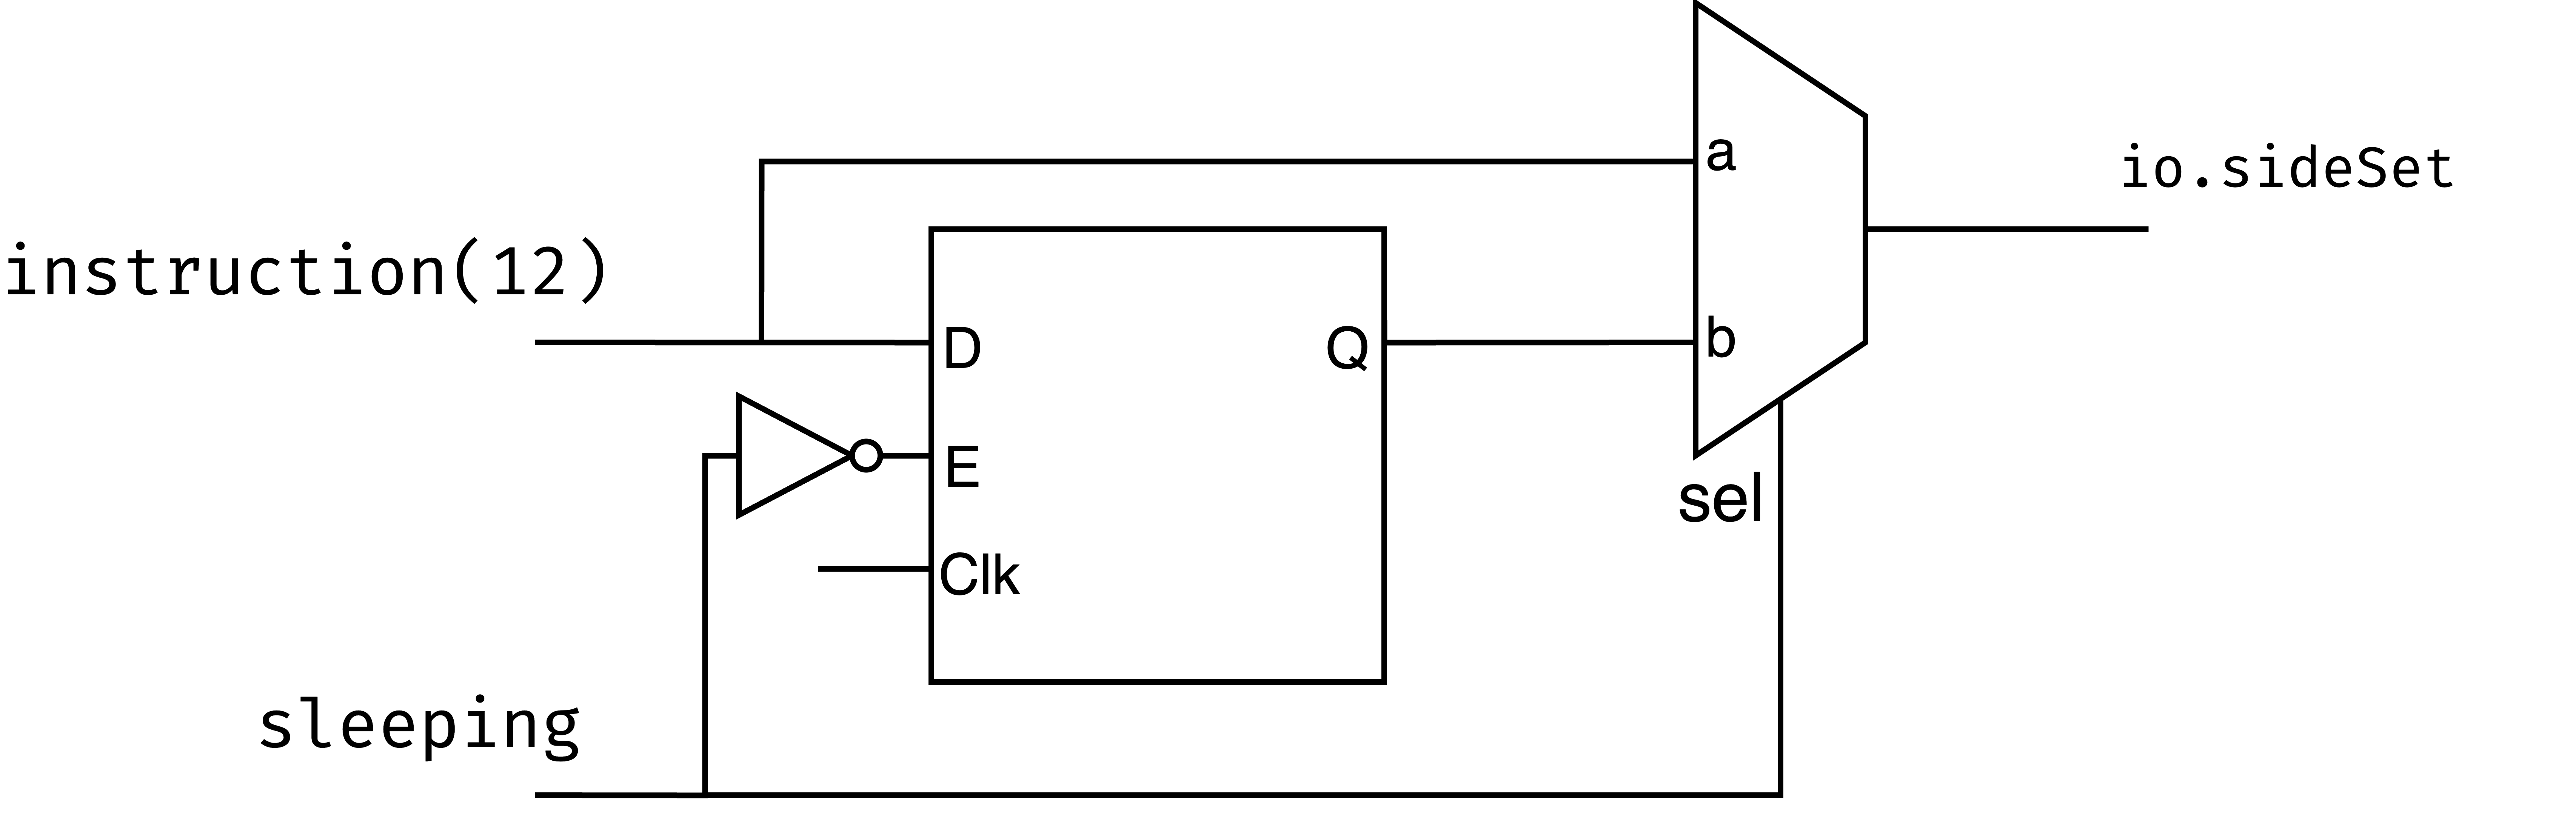
\includegraphics[width=0.9\textwidth]{../img/side-set.png}
    \caption{Logic for latching side-set}
    \label{fig:side-set}
\end{figure}

\begin{listing}[h!]
    \vspace{0.5cm}
    \begin{minted}{scala}
val sideSet    = instruction(12)
val sideSetReg = RegEnable(
    next = sideSet, 
    init = false.B, 
    enable = !sleeping
)
io.sideSet := Mux(sleeping, sideSetReg, sideSet)
    \end{minted}
    \caption{Chisel code for latching side-set}
    \label{lst:side-set}
\end{listing}



\subsection{Shift Registers}

The two shift registers, input and output, are fairly complex: they include logic for reading/writing from/to the FIFOs, as well as logic for shifting bits in and out. There are multiple configuration options too: shift direction, auto push/pull, shift thresholds, etc.


\subsubsection{OSR}

The OSR is the more complicated of the two, as autopull behaves slightly differently from autopush. Hence, there are a number of cases to handle for each instruction which interacts with the OSR.

A \txt{PULL} instruction will cause the OSR to be refilled, and the shift counter to be reset to 0, indicating the OSR is full. If a \txt{PULL} instruction has the `If Empty' flag set, then the pull only takes effect if the shift threshold has been reached, ie, the OSR is empty. If autopull is enabled and the OSR is full, then a \txt{PULL} instruction has no effect.

If an \txt{OUT} instruction is issued, autopull is enabled, and the OSR is empty, then instead of executing an out, the hardware will pull from the fifo and stall, causing the \txt{OUT} to happen on the next cycle. This is because a it cannot \txt{PULL} and then \txt{OUT} the pulled data on the same cycle due to the deep combinational path this would create from the FIFOs straight to the outputs. An \txt{OUT} instruction otherwise shifts the register data in the configured direction by the specified number of bits, putting the N shifted out bits as the least significant bits on the 32-bit output line and filling the register with 0s. The shift count register is also incremented by N. After an \txt{OUT} instruction, an autopull may take place if the shift count register indicates threshold has been met (the OSR is empty) which causes the OSR to be refilled ready for the next \txt{OUT}.

\txt{MOVE} or \txt{SET} instructions may also read/write from the OSR. A read doesn't have any effect on the OSR or FIFO state, but a write to the OSR causes the shift count register to be reset to 0, indicating it has refilled.

This logic is implemented as a lot of chained/nested \txt{when}/\txt{otherwise} blocks, which makes for not the cleanest code and synthesises to a large multiplexer, but is the best way to represent the necessary logic. The shift counter value saturates at 32, which can be tricky to work with and hard to consistently get right, so a custom saturating addition operator \txt{+!} is used to perform the threshold checks and increments. Examples is shown in Listing \ref{lst:sat_add}.


\begin{listing}[h!]
    \vspace{0.5cm}
    \begin{minted}{scala}
//add shiftCount to the register, capping the value at 32.
shiftCountReg := shiftCountReg /+\ shiftCount
//boolean condition to check if shift count exceeds threshold
val thresholdReached = (shiftCountReg /+\ shiftCount) >= thresh
    \end{minted}
    \caption{Example usages of the saturating add operator}
    \label{lst:sat_add}
\end{listing}


scratch reg
read/write ports

\subsubsection{ISR}

The ISR is slightly simpler, as there are fewer implications in the interaction between a \txt{IN} instruction and autopush. An \txt{IN} instruction is similar to an \txt{OUT}: the data is shifted by N bits in the configured direction, and the N least significant bits of the input line are placed in the register (as the MSBs if shifting from the right, or LSBs if from the left).

A push may happen in parallel with a shift due to autopush if autopush is enabled and the autopush threshold is reached (the ISR is full). A \txt{PUSH} instruction has the same behaviour as an autopush: write a word to the FIFO and clear the register, resetting the shift count to 0. The `If Empty' flag behaves similarly to the `If Full' flag, only allowing a push to take place if the ISR is full. A push triggered either automatically or by an instruction may stall if the FIFO is full.

\subsection{FIFOs}

The FIFOs are capable of storing up to 4 32-bit words, and buffer data between the PIO system and the rest of the SoC. The complexity in the FIFOs lies in the fact that the PIO and the SoC operate in different clock domains, meaning the FIFOs must be asynchronous.

Using the TX FIFO as an example, the write end of the FIFO that data is queued into operates within the SoC clock domain, while the read end is within the PIO clock domain. We have to ensure that data consumed by the PIO is \textit{stable} when it is read. This leads to the issue of \textit{metastability}, a term that refers to signals which `do not assume stable 0 or 1 states for some duration of time at
some point during normal operation of a design' \cite{cdc}. Appropriate synchronisation techniques are required to ensure that FIFO data is valid when read.

The asynchronous FIFO design we use from the paper `Simulation and Synthesis Techniques for Asynchronous FIFO Design' by Cummings \cite{fifo1}. Two designs are published, one by Cummings in \cite{fifo1} and another that builds upon the first by Cummings \& Alfke in \cite{fifo2}, both detailing asynchronous FIFO designs with full Verilog source lisings. We utilise the first one and translate the code from Verilog to Chisel, as the FIFO design described is able to be constructed within the constraints imposed by Chisel's implicit clocking model.

The FIFOs work is using a read and a write pointer that index into a shared memory and are used to detect if the FIFO is full or empty. The (TX FIFO) read pointer exists in the PIO clock domain and the write pointer in the SoC clock domain. To signal to the PIO that the FIFO is empty, or to the SoC that the FIFO is full, each pointer must be synchronised into the other domain to generate the full/empty signals.

Using binary counters in asynchronous FIFO designs can cause issues, as an increment can cause multiple signals to change (ie, 7 to 8 is 0111 to 1000). To overcome this, Gray code counters are used, where neighbouring numbers only differ by a single binary digit, which overcomes issues with synchronising multiple simultaneous signal changes accross clock domains.

Possibly the simplest synchronisation technique is used: the two flip-flop synchroniser. The way this works is using two flip flops both clocked in the domain that the signal is being synchronised into. The first flip-flop samples the input signal into the new clock domain and adds a cycle of delay to allow any metastability to decay. The second flip-flop samples from the first, with the idea that the output of the second one is a stable and valid signal \cite{cdc}. The circuit is shown in Figure \ref{fig:2ff}, and the (very succinct) chisel implementation is given in Listing \ref{lst:2ff}.

\begin{figure}[H]
    \centering
    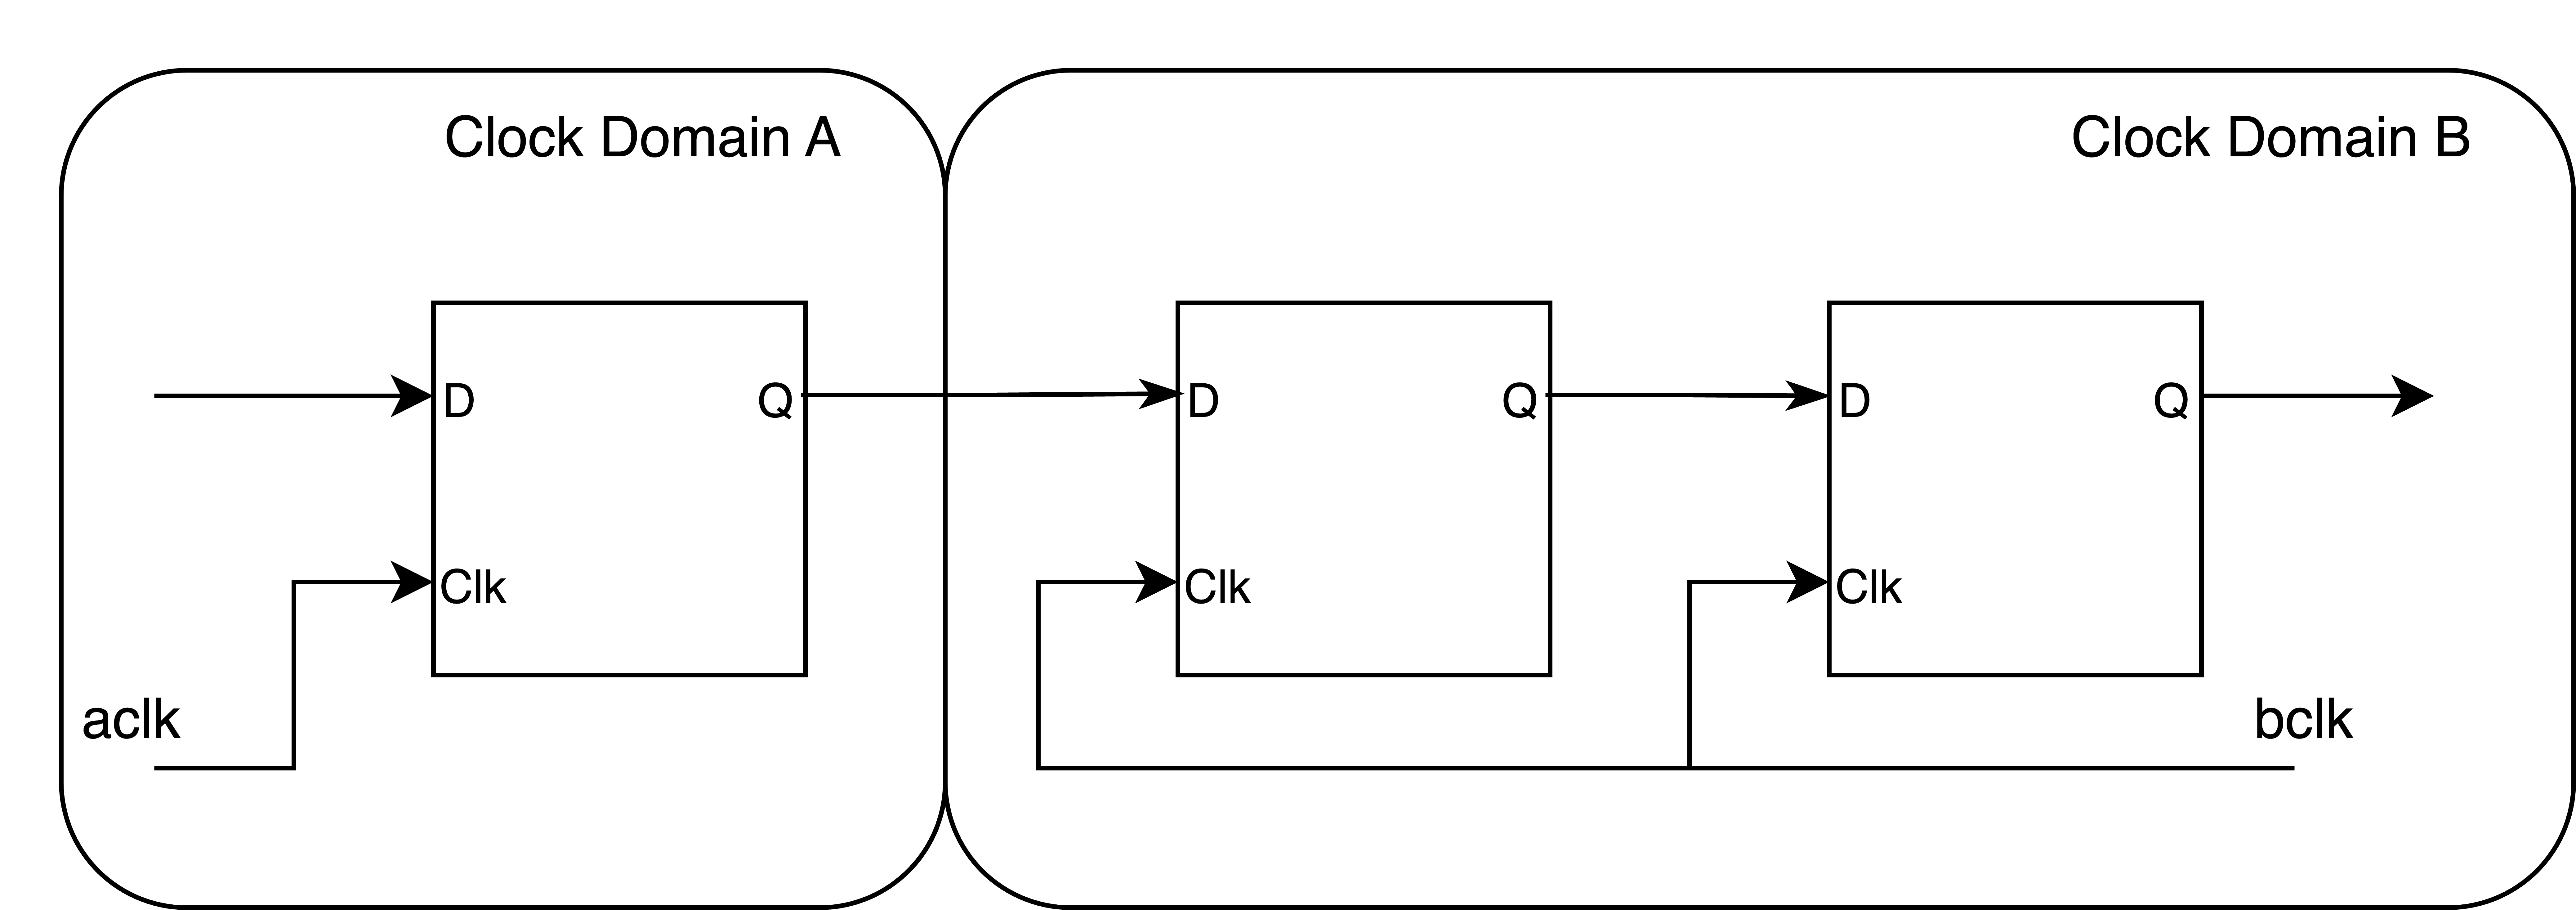
\includegraphics[width=\textwidth]{../img/2ff.png}
    \caption{A 2 flip-flop synchroniser \cite{cdc}.}
    \label{fig:2ff}
\end{figure}

\begin{listing}[h!]
    \vspace{0.5cm}
    \begin{minted}{scala}
object Synchroniser {
    def apply(input: UInt) = RegNext(RegNext(inputPointer))
}        
    \end{minted}
    \caption{Chisel code implementing a 2 flip-flop synchroniser using \txt{RegNext} objects.}
    \label{lst:2ff}
\end{listing}

There is a control module in both the read and write clock domains to generate the read/write Gray code pointer, read/write address (in binary) and empty/full signals. The write control module takes as input the read pointer synchronised into the writer clock domain and the \txt{doWrite} input signal. It computes the write address in binary, the write Gray code pointer, and asserts the \txt{full} output if necessary. The converse exists for the read side of the FIFO.

The top-level module has a clock and reset input for either side, as well as a producer/consumer IO bundle, shown in Listing \ref{lst:fifobundles}. The FIFO module is a Chisel \txt{RawModule}, meaning it does not have an implicit clock or reset and does not exist in any clock domain by default. Instead, \txt{withClockAndReset} helper objects are used to explicitly declare clock domains for either side of the FIFO, within which the control and synchronisation modules for either side are generated, shown in Listing \ref{lst:fifo}.

\begin{listing}[h!]
    \vspace{0.5cm}
    \begin{minted}{scala}
// a producer writes to the FIFO
class ProducerIO extends Bundle {
    val write   = Input(UInt(32.W))
    val doWrite = Input(Bool())
    val full    = Output(Bool())
}

// a consumer reads from the FIFO
class ConsumerIO extends Bundle {
  val read   = Output(UInt(32.W))
  val doRead = Input(Bool())
  val empty  = Output(Bool())
}

class AsyncFifoIO extends Bundle {
  val producerClock = Input(Clock())
  val producerReset = Input(Reset())
  val producer      = new ProducerIO

  val consumerClock = Input(Clock())
  val consumerReset = Input(Reset())
  val consumer      = new ConsumerIO
}
    \end{minted}
    \caption{FIFO interface bundles.}
    \label{lst:fifobundles}
\end{listing}


\begin{listing}[h!]
    \vspace{0.5cm}
    \begin{minted}{scala}
class AsyncFifo extends RawModule {
    val io = IO(new AsyncFifoIO)
    
    // shared wires that are used in both domains
    val readAddress  = Wire(UInt(2.W))
    val writeAddress = Wire(UInt(2.W))
    val readPointer  = Wire(UInt(3.W))
    val writePointer = Wire(UInt(3.W))
    
    val mem = Mem(4, UInt(32.W))
    
    withClockAndReset(io.producerClock, io.producerReset) {
        val write = Module(new WritePointer)
        // write connections and logic logic ...
    }
    
    //read clock domain (consumer)
    withClockAndReset(io.consumerClock, io.consumerReset) {
        val read = Module(new ReadPointer)
        // read connections and logic ...
    }
}
    \end{minted}
    \caption{FIFO interface bundles.}
    \label{lst:fifo}
\end{listing}

\subsection{Pin Mapping}

Pin mapping in RVPIO is much simplified from that of the RP2040. This is due in part to the fact that an RP2040 PIO block includes 4 state machines which share the pins via a priority mask that determines which state machine has access to which pin, whereas we only have a single state machine. The RP2040 also includes the ability for PIO programs to change the pin directions by writing data to a special `pindirs' register, instead of it being fixed by configuration registers, a feature also not present in RVPIO.

The 32-bit vector that represents the physical pins on the FPGA device is both an input and an output, requiring the use of a Verilog \txt{inout} port. Chisel does not provide support for working with bi-directional or analog logic types, so the pin mapping module is instead written in Verilog and wrapped using Chisel's `Black Box' functionality. Listing \ref{lst:blackbox} shows how Chisel can wrap external Verilog code for interoperability between Chisel and Verilog, with the \txt{Pins} class usable as a regular Chisel module within other Scala code.

\begin{listing}[h!]
    \centering
    \vspace{0.5cm}
    \begin{minted}{scala}
class Pins extends BlackBox with HasBlackBoxResource {
    val io = IO(new PinsIO)
    addResource("vsrc/Pins.v")
}
    \end{minted}
    \caption{Wrapping a Verilog module from another file as a Chisel module. The \txt{PinsIO} definition is omitted for brevity.}
    \label{lst:blackbox}
\end{listing}

The module is required to take as input the configured input and output base and count, as well as have a 32-bit input port for writing data to pins and for the side set, and 32-bit output for data read from the pins. The config inputs are used to generate a mask to place the correct input bits on the output read line, as shown in Listing \ref{lst:in-mask}.

\begin{listing}[h!]
    \vspace{0.5cm}
    \begin{minted}{verilog}
//generate mask
wire [31:0] inMask  = (32'b1 << cfg_inCount)  - 32'b1; 
wire [31:0] inputData; //data from pins
//shift data to LSBs and mask off the number we want
assign read = (inputData >> cfg_inBase) & inMask; 
    \end{minted}
    \caption{Verilog for generating read data from pins}
    \label{lst:in-mask}
\end{listing}

For the outputs, similar logic is used, shown in Listing \ref{lst:out-mask}. The \txt{write_enable} input is high when data is to be written out to the pins, and the data sent to the module from the PIO system is masked and shifted to the correct bits of the output port before being latched into the register.

\begin{listing}[h!]
    \vspace{0.5cm}
    \begin{minted}{verilog}
wire [31:0] outMask = (32'b1 << cfg_outCount) - 32'b1;    
reg  [31:0] outputData;
always @ *
    if(write_enable)
        outputData = (write_data & outMask) << cfg_outBase;
    \end{minted}
    \caption{Verilog for generating read data from pins}
    \label{lst:out-mask}
\end{listing}

The \txt{outputData} register is written to the \txt{inout} pins port and the \txt{inputData} wire is sampled from it. To achieve this, bidirectional tri-state buffers are used, specifically IOBUF primitives present in the FPGA device. A diagram of the IOBUF, and how it maps the inputs and outputs to the I/O pad is shown in Figure \ref{fig:iobuf}.

\begin{figure}[H]
    \centering
    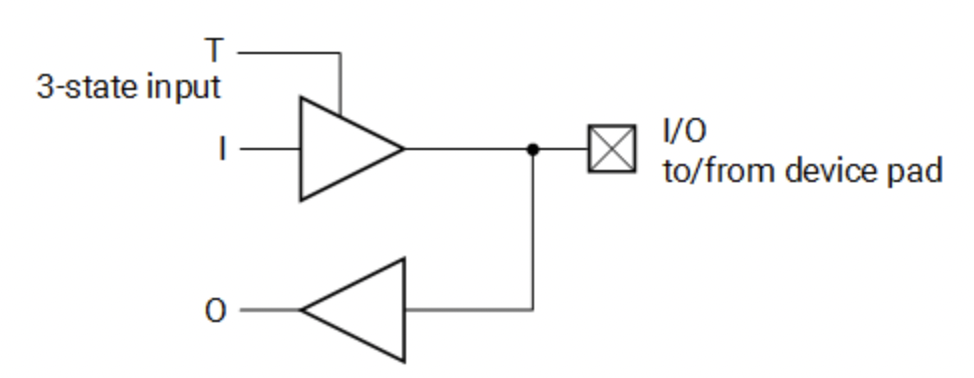
\includegraphics[width=0.9\textwidth]{../img/iobuf.png}
    \begin{tabular}{|c|c|c|c|}
        \hline
        \multicolumn{2}{|c|}{\textbf{Inputs}} & \textbf{Outputs} & \textbf{Bidirectional}               \\\hline
        \textbf{T}                            & \textbf{I}       & \textbf{O}             & \textbf{IO} \\\hline
        1                                     & X                & IO                     & Z           \\\hline
        0                                     & 1                & 1                      & 1           \\\hline
        0                                     & 0                & 0                      & 0           \\\hline
    \end{tabular}
    \caption{Xilinx IOBUF primitive \cite{vivado_libs}}
    \label{fig:iobuf}
\end{figure}

Xilinx provides Verilog macros for using primitives \cite{vivado_libs}. 31 single-bit IOBUFs are used in the design, instantiated within a generative for loop as shown in Listing \ref{lst:iobuf}, with the \txt{outputEnables} mask generated from the output config register. Pin 32 is always the side-set pin, so the most significant bit of the 32-bit output register is always disregarded, and the most significant 32-bit of the input wire is always 0.

\begin{listing}[h!]
    \vspace{0.5cm}
    \begin{minted}{verilog}
for(genvar i = 0; i < 31; i = i+1) begin
IOBUF #( 
    // output drive strength in mA
    .DRIVE(12), 
    // low Power - "TRUE", high Performance = "FALSE"
    .IBUF_LOW_PWR("TRUE"),  
    // I/O standard from constraints
    .IOSTANDARD("LVCMOS33"),
    //output slew rate 
    .SLEW("SLOW") 
) IOBUF_inst (
     // Buffer output (module data input)
    .O(inputData[i]),
    // Buffer inout port (module pins inout)     
    .IO(pins[i]),   
    // Buffer input (module data output)
    .I(outputData[i]),     
    // 3-state enable input, high=input, low=output
    .T(!outputEnables[i])     
);
end
    \end{minted}
    \caption{Instantiating IOBUFs in a loop in Verilog using Xilinx macros\cite{vivado_libs}}
    \label{lst:iobuf}
\end{listing}

\subsection{Clock Divider}

The clock divider was another module that had to be written in Verilog. FIRRTL does not provide support for generating clock dividers or clock multiplexers \footnote{\url{https://github.com/chipsalliance/firrtl/issues/540}} due to the special treatment clock signals get within Chisel and FIRRTL. The module takes the 16-bit divisor value and an input clock, and outputs a slowed clock. Listing \ref{lst:clockdiv} shows the black box module. Note how \txt{Clock} is it's own distinct type within Chisel, distinct from \txt{Bool}.

\begin{listing}[h!]
    \centering
    \vspace{0.5cm}
    \begin{minted}{scala}
class ClockDivider extends BlackBox with HasBlackBoxResource {
    val io = IO(new Bundle {
        val clock   = Input(Clock())
        val divisor = Input(UInt(16.W))
        val outClk  = Output(Clock())
    })
    addResource("vsrc/ClockDivider.v")
}
    \end{minted}
    \caption{The \txt{ClockDivider} black box module definition.}
    \label{lst:clockdiv}
\end{listing}

A companion object is used for the clock divider to enable functional module creation. Companion objects in Scala are objects declared in the same file as the class of the same name, and allow to add static methods and factory methods to the class. The \txt{apply} method is a special method in Scala that is used when calling an object like a method: \txt{Foo(bar)} desugars to \txt{Foo.apply(bar)} \cite{scala_book}.

In Chisel, this allows to add ways to instantiate modules that are more intuitive and readable hardware descriptions using the way Scala evaluates expressions. Listing \ref{lst:clockdiv2} shows the \txt{ClockDivider} companion object and it's \txt{apply} method, along with an example usage. The method returns the \txt{clkdiv.io.outClk}, meaning that in the example line below the \txt{slowClock} is the output of the clock divider. A similar technique is used to provide the \txt{Mux} and \txt{RegEnable} objects from Chisel's standard library shown in Lising \ref{lst:side-set}.

\begin{listing}[h!]
    \centering
    \vspace{0.5cm}
    \begin{minted}{scala}
object ClockDivider {
    def apply(divisor: UInt, clock: Clock): Clock = {
        val clkdiv = Module(new ClockDivider)
        clkdiv.io.clock := clock
        clkdiv.io.divisor := divisor
        clkdiv.io.outClk
    }
}
//example usage
val slowClock = ClockDivider(divisor, fastClock)
    \end{minted}
    \caption{The \txt{ClockDivider} companion object and example usage}
    \label{lst:clockdiv2}
\end{listing}

\section{SoC Integration}

As discussed in Chapter \ref{ch:objectives}, the Chisel design must be integrated into the SoC. The top-level PIO RTL module is compiled to Verilog and imported into Vivado as a design source. The module can then be included in the block diagram like any other RTL module or IP core for synthesis targeting the Xilinx FPGA.

\subsection{AXI-Lite Wrapper}

The block diagram in \ref{fig:bd} shows three external interfaces that need to be connected to the rest of the SoC: the RX FIFO producer, the TX FIFO consumer, and the instruction memory and control registers.

The latter is a single write-only address port, with the instruction memory mapped to addresses 0 to 31, and the control registers above that. To connect to the AXI network within the SoC, we implemented an AXI4-lite slave interface within Chisel and wrapped the top-level PIO module in it with the write data and address channels were connected to the write data port of the PIO.

AXI-Lite is suited best to this application as it is a much simpler interface than full AXI, best suited to simple memory-mapped registers such as this. It is interoperable with full AXI buses, making it easy to integrate \cite{axi}.

There are 5 channels in an AXI bus: read address, read data, write address, write data, and write response. Each one uses a ready/valid handshake for exchanging data, something which Chisel has utilities in it's standard library for working with. The \txt{Decoupled} class works similar to the \txt{ReadWrite} class discussed in Section \ref{sec:readwrite}, and adds a \txt{ready} input and \txt{valid} output to a Chisel \txt{Data} type. This can be used to build an AXI interface in Chisel quite nicely, using nested bundles for each of the channels

\begin{figure}[H]
    \centering
    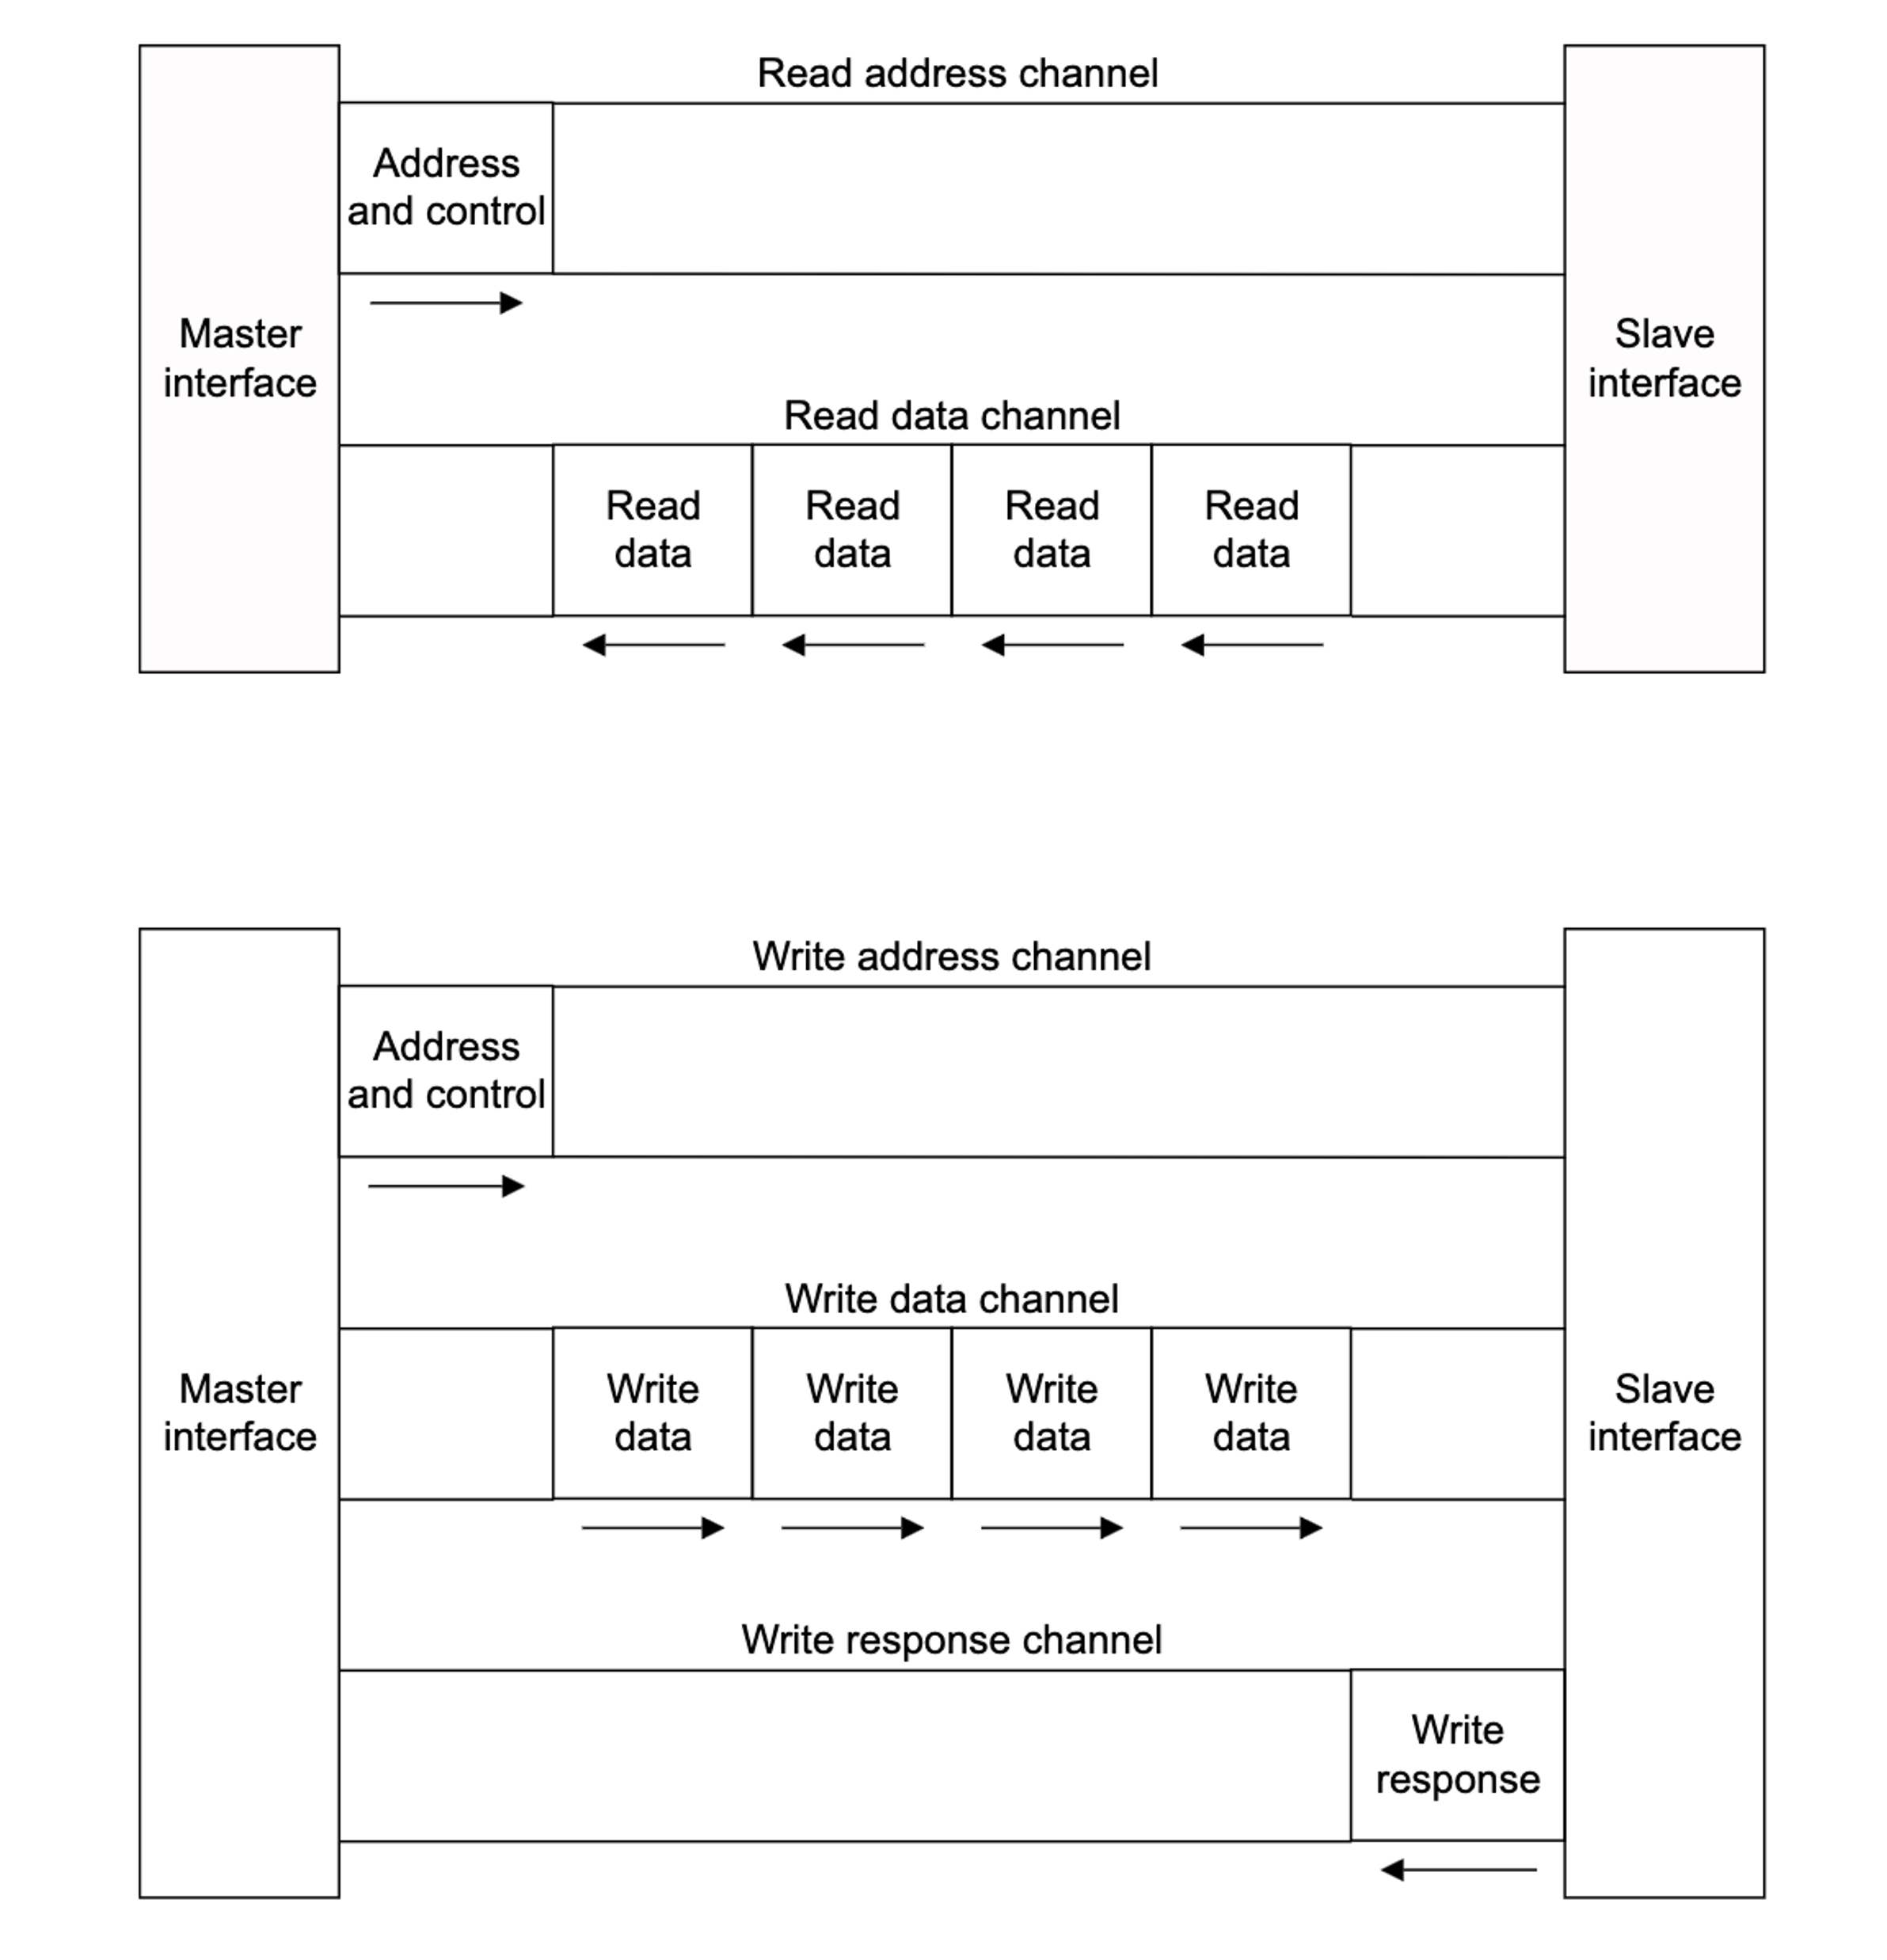
\includegraphics[width=0.7\textwidth]{../img/axi-chan.png}
    \caption{The 5 AXI communication channels}
    \label{fig:axi-chan}
\end{figure}

\begin{listing}[h!]
    \centering
    \vspace{0.5cm}
    \begin{minted}{scala}
class AXILiteAddress(addrWidth: Int) extends Bundle {
    val addr = UInt(addrWidth.W) 
    val prot = UInt(3.W) // transcation security level        
}   
class AXILiteWriteData(dataWidth: Int) extends Bundle {
    val data = UInt(dataWidth.W)
    val strb = UInt((dataWidth / 8).W)  // write strobing
}
class AXILiteReadData(dataWidth: Int) extends Bundle {
    val data = UInt(dataWidth.W)
    val resp = UInt(2.W) // status response
}
class AXILiteSlave(addrWidth: Int, dataWidth: Int) 
    extends Bundle {
    val readAddr = 
        Flipped(Decoupled(new AXILiteAddress(addrWidth)))   
    val readData = Decoupled(new AXILiteReadData(dataWidth))        
    val writeAddr = 
        Flipped(Decoupled(new AXILiteAddress(addrWidth)))  
    val writeData = 
        Flipped(Decoupled(new AXILiteWriteData(dataWidth)))
    val writeResponse = Decoupled(UInt(2.W))                             
}
    \end{minted}
    \caption{The \txt{ClockDivider} companion object and example usage}
    \label{lst:axi}
\end{listing}

The interface definition is parametrised such that it can be implemented for any address and data width, but the AXI-Lite specification allows for only 32-bit and 64-bit data words. The bus used is therefore 32-bit, but only the lower 16 bits of the word are used.

Vivado's block design tools recognise the exposed interface on the RTL module as an AXI-bus and allow to drag-and-drop connect it with the rest of the block design and interoperate with the rest of Xilinx's IP portfolio with ease.

\begin{figure}[h]
    \centering
    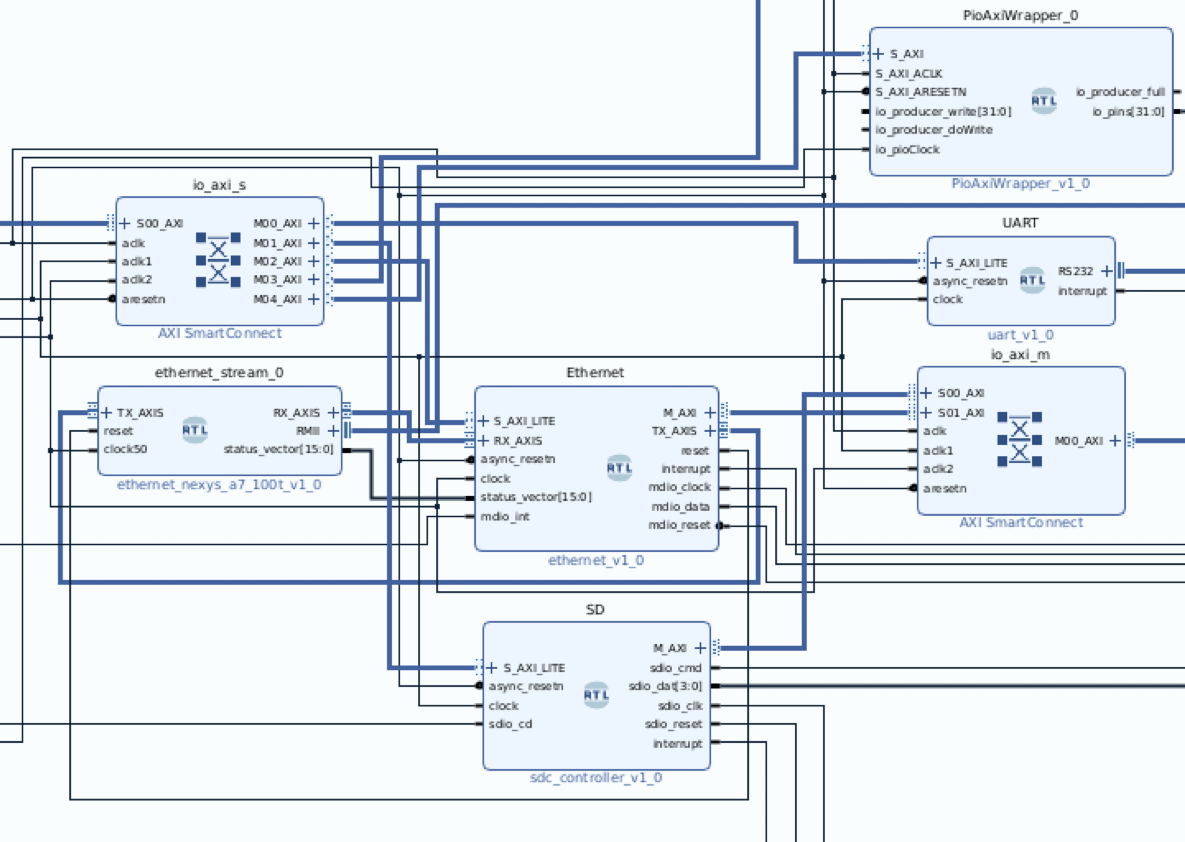
\includegraphics[width=1\textwidth]{../img/axi-net.png}
    \caption{The PIO block with it's AXI-Lite wrapper (top right) connected within Vivado's block design tools as part of an AXI network using Xilinx IP.}
    \label{fig:axi-net}
\end{figure}

\subsection{FIFOs, AXI-Stream \& DMA}
\label{sec:dma}

The FIFO interfaces would be connected using AXI-Stream to a DMA controller on the SoC. AXI-Stream allows to transfer a continuous stream of data via an AXI bus, and is more suitable than AXI-Lite or regular AXI for the FIFOs due to the need to continually stream data in bursts, as AXI is transaction-based and defines a maximum data transfer burst length \cite{axi_stream}.

It is possible to add a DMA device to Rocket Chip as a TileLink master device that is able to send it's own read and write requests to the memory system \cite{chipyard}. A TileLink DMA device with an external AXI-Stream master and slave port would need to be added to the Rocket Chip design to connect the FIFOs via this mechanism.

Unfortunately due to time and complexity constraints this interface was not added, and the PIO device as we present it is not able to stream data to or from the host system via the FIFOs.
